

\chapter{Convolution}

\section{Introduction}

\todo{Conv Intro} \textit{Conv Intro: To write it down later}.

\section{Definition}

The definition of convolution between 2 signals $x$ and $h$ is:

\begin{equation}
\begin{array}{rcl}

y(t) \, &=& \, \displaystyle \int_{-\infty}^{+\infty} x(\tau) \, h\left(\,t \, - \tau\, \right) d \tau \\ \\

y[k] \, &=& \, x[k] \, * \, h[k] \\ \\
 &=& \displaystyle\sum_{m \, = \, - \, \infty}^{+ \, \infty} x[m] \, h[k \, - \, m] 		
\end{array}
\label{Eq:conv:formula}
\end{equation}

\underline{Notes for \autoref{Eq:conv:formula}:}

\begin{itemize}

\item $h\left(\,t \, - \tau\, \right)$: there is an inversion with respect to time axis (the $-$), then a delay by $t$

    \begin{itemize}
    \item  The integration is with respect to $\tau$, so $\tau$ is the time axis

    \item  The inversion with respect to time, that is  $h(-\tau)$, we flip $h(\tau) \rightarrow$ we have a symmetry (mirror) with respect to $y$ axis
    \end{itemize}

\item  So the shifting will be with respect to $t$ or $m$ in discrete time case: it can be $< \, 0$ or $> \, 0$

    \begin{itemize}
    \item To evaluate the $\displaystyle\int$ or $\displaystyle\sum$ in \autoref{Eq:conv:formula}, we need to take all shifting cases
    \end{itemize}

\end{itemize}

\newpage
\section{Properties}

\underline{Width Property:}\\

$h_1[k]$ has a length of $m_{h_1}$ and $h_2[k]$ has a length of $m_{h_2}$, the resultant signal will have a length of $m_{h_1}  \, + \,m_{h_2} \, - \, 1 $.\\


\underline{Start and Stop time:}\\

\begin{itemize}

\item Start time of $y[k] \, = \, $ start of $x \, + \,$ start of $h$

	\begin{itemize}
	\item Where the start of $x$ and start of $h$ is from the non zero values
	\end{itemize}

\item Stop time of  $y[k] \, = \, $ stop of $x \, + \,$ stop  of $h$

	\begin{itemize}
	\item Where the stop t of $x$ and stop  of $h$ is from the non zero  values
	\end{itemize}

\end{itemize}

\newpage
\section{Example in Continuous Time}

\subsection{Example 1}
\label{sub:ex1_convolution}

Given is shown in \autoref{fig:Convolution:ex1_cont_time}

\begin{figure}[h]
\centering
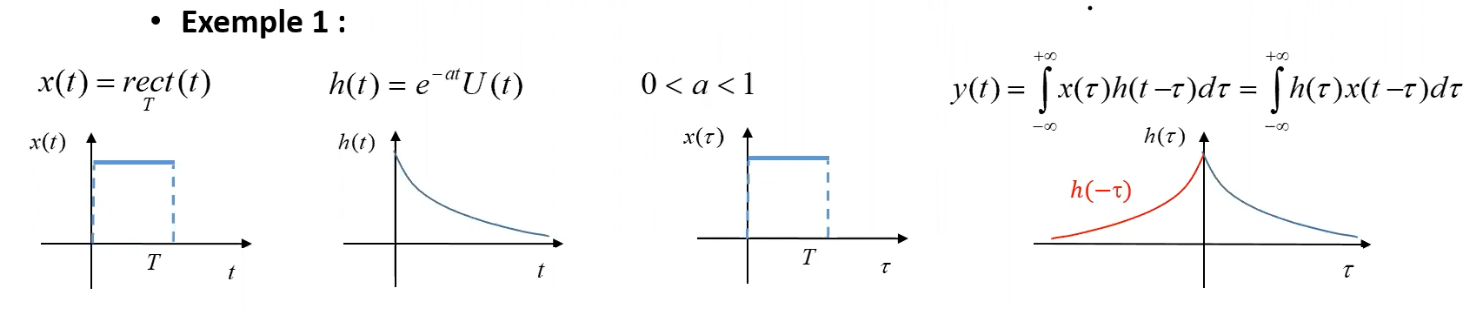
\includegraphics[width = 1.0\textwidth, frame]{Figures/Convolution/ex1_cont_time}
\caption{Example 1 given}
\label{fig:Convolution:ex1_cont_time}
\end{figure}

Before solving, some comments regarding the example:

\begin{itemize}

\item The signal $x(t)$ is time shifted with respect to $T$, it's not like the standard rect function which starts from $\displaystyle\frac{-T}{2} \rightarrow \displaystyle\frac{T}{2}$

\item  Remember that now the new time axis is $\tau$ and not $t$.

    \begin{itemize}
        \item $t$ will act as some constant which can have different cases
    \end{itemize}

\end{itemize}

Now to solve this example, we need to study different time shift cases for $h(\tau)$, but after inversion, that is shifting for $h(-\tau)$. The shifting cases are illustrated in \autoref{fig:Convolution:ex1_time_shift_cases}.

\begin{figure}[h]
\centering
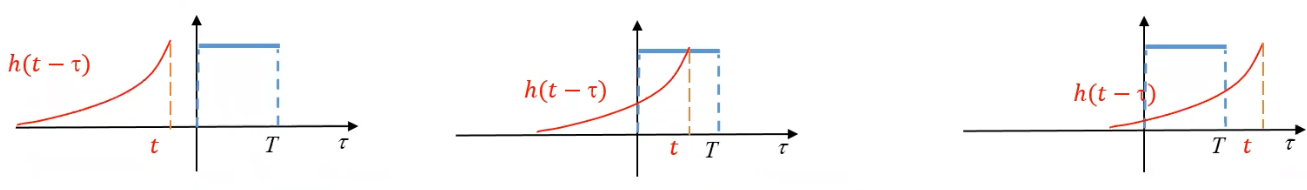
\includegraphics[width = 1.0\textwidth, frame]{Figures/Convolution/ex1_time_shift_cases}
\caption{Example 1 time shifting cases}
\label{fig:Convolution:ex1_time_shift_cases}
\end{figure}

\begin{itemize}

\item Tor $t \, < \, 0$: there is no common area between $x$ and $h$, so $y(t) \, = \, 0$ for $t \, \leq \, 0$

\item  For $t \, > \, 0$:  the signal $x$ finishes at a duration $T$, but $h$ can continue beyond $T$, so in case of $>0$, we distinguish 2 cases: 

    \begin{enumerate}
    \item $0 \,<\, t \, < \, T$:  the boundaries of common surface is from $\tau \, = \, 0 \rightarrow \, \tau \, = \, t$. Using \autoref{Eq:conv:formula}, we have:


$\begin{array}{rcl}
     y(t) &=& \displaystyle \int_{-\infty}^{+\infty} x(\tau) \, h\left(\,t \, - \tau\, \right) d \tau  \\ \\
      &=& \displaystyle \int_{0}^{t} 1 \, \times \, e^{-a \, (t \, - \, \tau)} \, d \tau
\end{array}$

Since the integration is with respect to $\tau$, we can all the non $\tau$ variables ($t$ and $a$) act as constant and we can get them out of the integral

\newpage
$\begin{array}{rcl}
 y(t) &=& e^{-a \, t} \displaystyle \int_{0}^{t} e^{a \, \tau} d\tau \,   \\ \\
    &=& e^{-a \, t}  \left[ \displaystyle\frac{e^{a\tau}}{a} \right]_{0}^{t} \\ \\ 
    &=& \displaystyle\frac{e^{-a \, t}}{a} \, (e^{a \, t} \, - \, 1) \\ \\ 
    &=& \, \displaystyle\frac{1}{a} \, \times \, \left[ \,e^{-a \, t} \, \times \, \left( \, e^{at} \, - \, 1 \,\right) \, \right] \\ \\
    &=& \displaystyle\frac{1}{a} \, \left(\, 1 \, - \, e^{-a \, t}   \, \right)
    
\end{array} $\\

\item  $t \, > \, T$: in this case the common area from $\tau \, = \, 0 \rightarrow \, \tau \, = \, T$

Solving we get:\\

$\begin{array}{rcl}
y(t) &=& \displaystyle \int_{-\infty}^{+\infty} x(\tau) \, h\left(\,t \, - \tau\, \right) d \tau  \\ \\
    &=& \displaystyle \int_{0}^{T}  1 \, \times \, e^{-a \, (t \, - \, \tau)} \, d \tau \\ \\
    &=& e^{-a \, t}  \left[ \displaystyle\frac{e^{a\tau}}{a} \right]_{0}^{T} \\ \\ 
    &=& \, \displaystyle\frac{e^{-a \, t}}{a} \, (e^{a \, T} \, - \, 1)
\end{array}$

Rearranging the constant terms we get:


$\begin{array}{rcl}

y(t) \, = \, \left(\, \displaystyle\frac{e^{a \, T} \, - \, 1}{a} \,\right) \, \times \, e^{-a \, t} \text{ for } t \, > \, T

\end{array}$    
    \end{enumerate}

    
\end{itemize}

As a recap, the solution is:

\begin{equation}
y(t) \, = \, 
\begin{cases}
       0 \quad \text{for } t \, < \, 0  \\ \\
        \displaystyle\frac{1}{a} \, \left(\, 1 \, - \, e^{-a \, t}   \, \right) \quad \text{for } 0 \, < \, t \, < T \\ \\
        \left(\, \displaystyle\frac{e^{a \, T} \, - \, 1}{a} \,\right) \, \times \, e^{-a \, t} \text{ for } t \, > \, T
\end{cases} 
\end{equation}



\newpage
\subsection{Example 2}

\underline{Given:} compute the convolution between $x(t)$ and $h(t)$ given in \autoref{Eq:conv:given_ex2}

\begin{equation}
\begin{array}{rcl}
     x(t) &=& \text{some signal}  \quad t \, \in \, ]- \infty \, ,\, - \infty  [   \\ \\
    h(t) &=& \,  \displaystyle\frac{1}{T} \, \text{rect(t)} \quad t \in \left[ \displaystyle\frac{-T}{2} \, , \, \displaystyle\frac{T}{2}  \right]
\end{array}
\label{Eq:conv:given_ex2}
\end{equation}




\underline{Solution:}\\

The signal $x(t)$ is assumed to be some general signal, and the only information we have is the that $x(t)$ exist for all value of $t$.

As for $h(t)$, it is centered at $t \, = \, 0$ , and has a duration $T$ from $\displaystyle\frac{-T}{2} \, \rightarrow \, \displaystyle\frac{T}{2}$.\\

The $\mathrm{1}^\mathrm{st}$ step is always as seen in \ref{sub:ex1_convolution} is the time inversion of $h(\tau)$ with respect to the $y$ axis. Since we have a $\text{rect}(t)$ signal, the inversion will result in the same signal since the rect signal is already symmetric with respect to the $y$ axis.\\

After we have $h(-\tau)$, we start shifting it with different values of $t$. In other words, $h(-\tau)$ is centered at 0, now it will be centered at $t$, and the $t$ can be $< \, 0$ or $>\, 0$, as shown in \autoref{fig:Convolution:rect_shifted}. 

\begin{figure}[h]
\centering
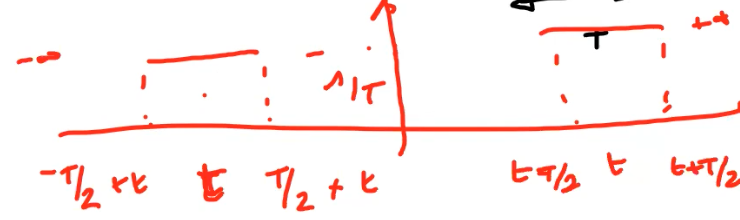
\includegraphics[width = 0.9\textwidth, frame]{Figures/Convolution/rect_shifted}
\caption{Shifting rect signal with different $t$ values}
\label{fig:Convolution:rect_shifted}
\end{figure}

\newpage
Applying \autoref{Eq:conv:formula} for different values of $t$ give the following cases:\\

\underline{$t \, < \, 0$}:


$\begin{array}{rcl}
 y(t) \, &=& \, \displaystyle \int_{-\infty}^{+\infty} x(\tau) \, h\left(\,t \, - \tau\, \right) d \tau  \\ \\
     &=& \, \displaystyle \int_{- \frac{-T}{2} \, + \,t}^{\frac{T}{2} \, + \,t} x(\tau) \, \times \displaystyle\frac{1}{T} \, \times \, 1 \, d\tau \\ \\
     &=& \, \displaystyle\frac{1}{T} \, \int_{- \frac{-T}{2} \, + \,t}^{\frac{T}{2} \, + \,t} x(\tau) \, d\tau
\end{array}$

\underline{$t \, > \, 0$}:\\

For $t \, > \, 0$, we have the same computation since the integral bounds will be the same.\\

The expression $ \displaystyle\frac{1}{T} \, \int_{- \frac{-T}{2} \, + \,t}^{\frac{T}{2} \, + \,t} x(\tau) \, d\tau$ is similar to taking the average of a signal $x(t)$. Recall that the average of a signal $x(t) \, = \, \displaystyle\frac{1}{T} \, \int_{-\frac{-T}{2}}^{\frac{T}{2}} x(t) \, dt$.

So we can say that $\displaystyle\frac{1}{T} \, \int_{- \frac{-T}{2} \, + \,t}^{\frac{T}{2} \, + \,t} x(\tau) \, d\tau$ is taking the average but with different values of $t$. 

That's why $\displaystyle\frac{1}{T} \, \text{rect(t)}$ is called an average filter, since the result of the filtering is taking the average of signal $x(t)$ for all values of $t$.\\

\underline{Note:} see simulation in \verb|MATLAB|.

\newpage
\section{Examples in Discrete Time}

\subsection{Finite Short Signals}
\label{Sub:TimeDomainDiscrete:Example_Short_Signlas}

To do later.


\subsection{Long or Infinite Signal Approach}

In the example of \autoref{Sub:TimeDomainDiscrete:Example_Short_Signlas}, the signals were having few values for some indexes, so the definition of equation (\ref{Eq:conv:formula}) were applicable and we can compute $c[k]$ for each $k$ index. But what if we have some long signals, or some infinite duration signals ? we need a more applicable approach.\\


The method is called \tbi{sliding tapes approach}, where it consist to shift $h[k]$ along the index axis, and compute the $c[k]$ for each time we do the shifting of $h[k]$. The sliding tapes approach can be summarized by doing the following steps:

\begin{enumerate}

\item Plot $f[k]$ and $h[k \, - \, m]$.

\item Shift $h[k \, - \, m]$ to far to the left (large $k$).

\item Multiply and Sum Signals (do the dot product).

\item Shift $k$ until new intermediate signal results.

\item Repeat 3 and 4 until done.

\end{enumerate}

\underline{Example 1:}\\

Let's compute the convolution between:

\begin{itemize}
\item $x[k] \, = \, \alpha^k \, u[k]$, where $0 \, \leq \, \alpha \, \leq \, 1$, so its a damping exponential.

\item $h[k] \, =  \, u[k]$.
\end{itemize}

First, let's recall the definition: $ x[k] \, * \, h[k] \, 
 = \displaystyle\sum_{m \, = \, - \, \infty}^{+ \, \infty} x[m] \, h[k \, - \, m] $.\\

\newpage
We need to able to sketch $x[m]$ and $h[k \, - \, m]$. The sketch is shown in \autoref{fig:Convolution:Example_1_SlidingTapes}.

\begin{figure}[h]
\centering
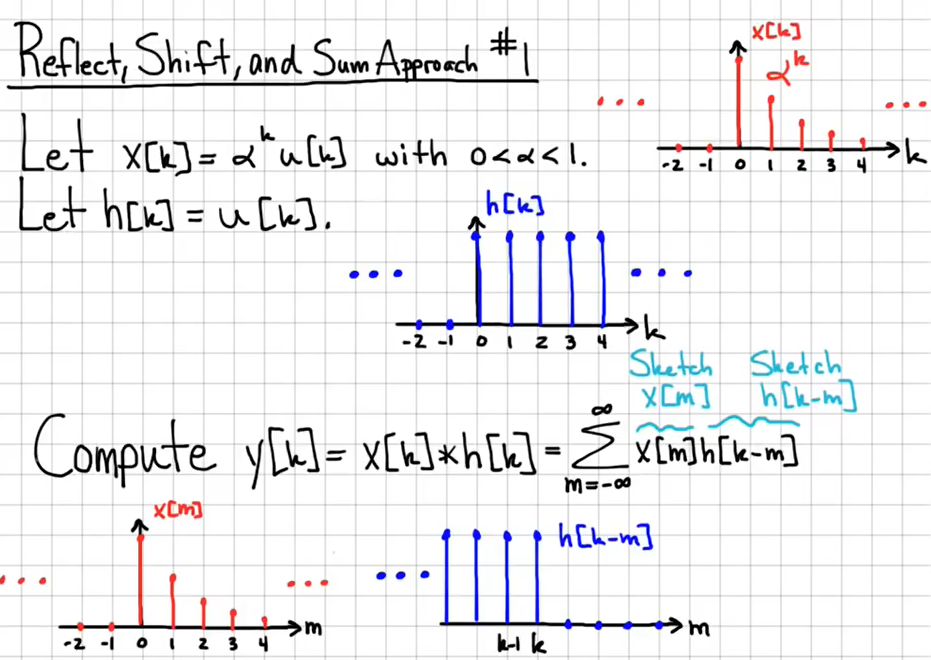
\includegraphics[width = 0.7\textwidth, frame]{Figures/Convolution/Example_1_SlidingTapes}
\caption{Sketching $x[m]$ and $h[k \, - \, m]$}
\label{fig:Convolution:Example_1_SlidingTapes}
\end{figure}

\begin{itemize}

\item $x[m]$ is quite easy because is the same as $x[k]$

\item $h[k \, - \, m]$ is the tricky one: it is a time reversed then shifted signal

	\begin{itemize}
	\item We first do time reversing, so the $h[-m]$ part (reflection with respect to the y axis.)
	
	\item Then we shift to the left
	\end{itemize}

\end{itemize}

The difference between $h[k \, - \, m]$ and $h[k]$ is that:

\begin{itemize}
\item $h[k]$ will turn on at $k \, = \, 0$ and still on until some $k$ value

\item $h[k \, - \, m]$ will be turned off at $k$, so it is the opposite of $h[k]$.
\end{itemize}

It is very important when plotting $h[k \, - \, m]$ to let $k$ be a variable, notice that in \autoref{fig:Convolution:Example_1_SlidingTapes} we didn't specify the origin of $h[k \, - \, m]$, we let it, because for each value of $k$, we will have a different $h[k \, - \, m]$.\\

\newpage
We will study the cases for 2 cases: $k \, < \, 0 $, where we take as example $k \, = \, -2$, and $k \, \geq \, 0$, where $k \, = \, 2$. These cases are shown in \autoref{fig:Convolution:Example_1_SlidingTapes_K_Cases}.

\begin{figure}[h]
\centering
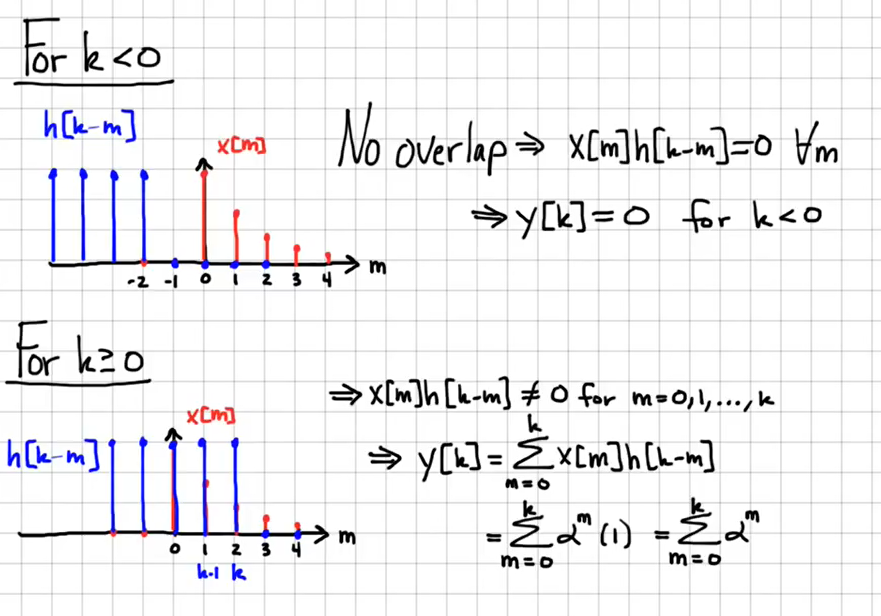
\includegraphics[width = 0.7\textwidth, frame]{Figures/Convolution/Example_1_SlidingTapes_K_Cases}
\caption{$h[k \, - \, m]$ for $k \, < \, 0 $ and $k \, \geq \, 0$}
\label{fig:Convolution:Example_1_SlidingTapes_K_Cases}
\end{figure}

\begin{itemize}

\item For any $k \, < \, 0 $, there will be no overlapping between $h[k \, - \, m]$ and $x[m]$, so the result of the convolution will be 0 for $k \, < \, 0 $.

\item For $k \, \geq \, 0$, there is overlapping between the 2 signals, and this overlapping stop till $k$, so the upper limit of the summation will be till $m \, = \, k$ instead of $m \, = \, + \infty$.

	\begin{itemize}
	\item And sine $x[m] \, = \, 0$ for $m \, < \,0$, so the lower limit of the summation will start from $m \, = \, 0$ instead of $m \, = \, - \infty$.
\end{itemize}	

For  $k \, \geq \, 0$, $h[k \, - \, m] \, = \, 1$.

\end{itemize}


The series for $k \, \geq \, 0$ can be solved using the following formula:

\begin{equation}
\displaystyle\sum_{n \, = \,0}^{N \, - \, 1} \alpha^n \, = \, \begin{cases}
N \quad \text{for } \alpha \, = \, 1 \\ \\
\displaystyle\frac{1 \, - \, \alpha^N}{1 \, - \, \alpha} \quad \text{any complex } \alpha\, \neq \, 1
\end{cases}
\label{Eq:Convolution:Series_Formula}
\end{equation}

\newpage
The computation are shown in \autoref{fig:Convolution:Example_1_SlidingTapes_y}, along with final answer of the convolution $y[k]$.

\begin{figure}[h]
\centering
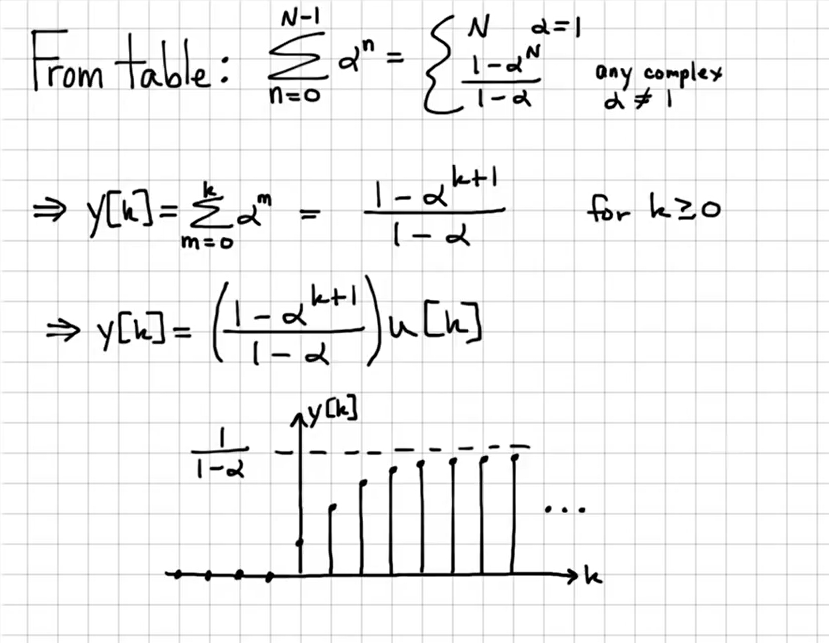
\includegraphics[width = 0.7\textwidth, frame]{Figures/Convolution/Example_1_SlidingTapes_y}
\caption{$y[k]$}
\label{fig:Convolution:Example_1_SlidingTapes_y}
\end{figure}

Notice that when computing $y[k]$, we add $+1$ to $k$, because the formula of equation (\ref{Eq:Convolution:Series_Formula}) add plus 1 to the upper limit $\left( \, N \, - \, 1 \, \right)$. Also the signal $y[k]$ converge to the limit $\displaystyle\frac{1}{1 \, - \, \alpha}$ as $k \, \rightarrow \, + \, \infty$.\\


\underline{Example 2:}\\

Example 2 is shown in \autoref{fig:Convolution:Example_2_SlidingTapes}.

\begin{figure}[h]
\centering
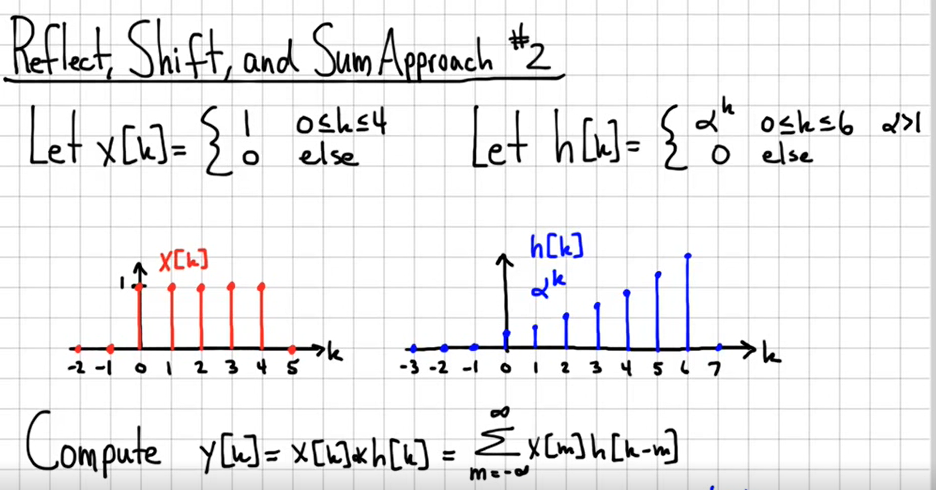
\includegraphics[width = 0.7\textwidth, frame]{Figures/Convolution/Example_2_SlidingTapes}
\caption{Question for Example 2}
\label{fig:Convolution:Example_2_SlidingTapes}
\end{figure}

\newpage
First step is to plot $x[m]$ and $h[k \, - \, m]$. The plot is shown in \autoref{fig:Convolution:Example_2_SlidingTapes_Sketching}.

\begin{figure}[h]
\centering
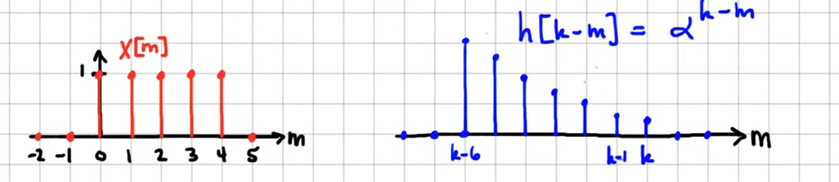
\includegraphics[width = 0.7\textwidth, frame]{Figures/Convolution/Example_2_SlidingTapes_Sketching}
\caption{Sketching $x[m]$ and $h[k \, - \, m]$}
\label{fig:Convolution:Example_2_SlidingTapes_Sketching}
\end{figure}

Again, $h[k \, - \, m]$ is time reversed first and then shifted to the left. We let $k$ to be a variable, and we will study different cases for $k$. Notice that $h[k \, - \, m]$ now start at index $m \, = \, k \, - \, 6$ and stop for index $m \, = \, k$.\\

The approach to compute the solution is the same as in example 1, but here we have more cases to be considered for $k$. All the cases are shown  below from \autoref{fig:Convolution:Example_2_SlidingTapes_Cases_1}  $\rightarrow$ \autoref{fig:Convolution:Example_2_SlidingTapes_Cases_3}.\\


\begin{figure}[h]
\centering
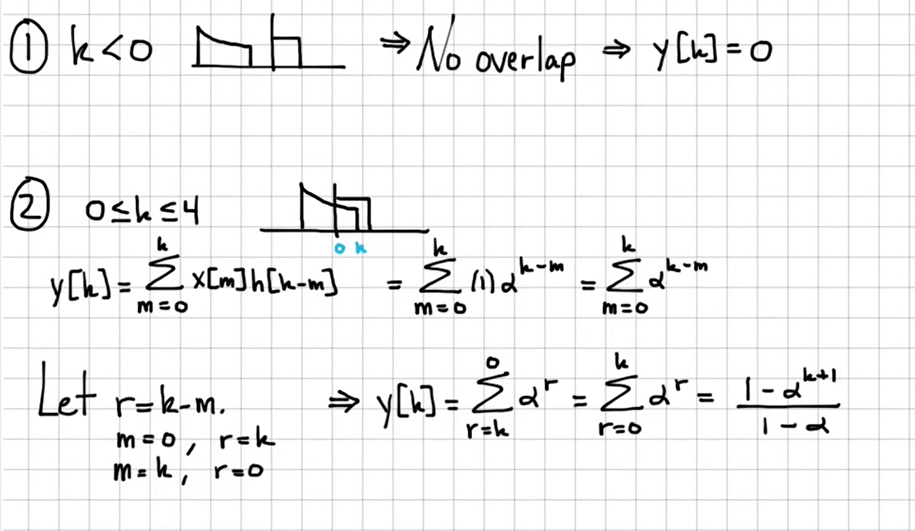
\includegraphics[width = 0.7\textwidth, frame]{Figures/Convolution/Example_2_SlidingTapes_Cases_1}
\caption{$k \, < \, 0$ and $0 \, \leq \, k \, \leq \, 4$}
\label{fig:Convolution:Example_2_SlidingTapes_Cases_1}
\end{figure}


\newpage
In \autoref{fig:Convolution:Example_2_SlidingTapes_Cases_1}, we have made a change of variable $r \, = \, k \, - \, m$ so we can use equation (\ref{Eq:Convolution:Series_Formula}), and also flip the order of series from $\displaystyle\sum_{r \, = \, k}^0 \, \rightarrow \, \displaystyle\sum_{r \, = \, 0}^k$.


\begin{figure}[h]
\centering
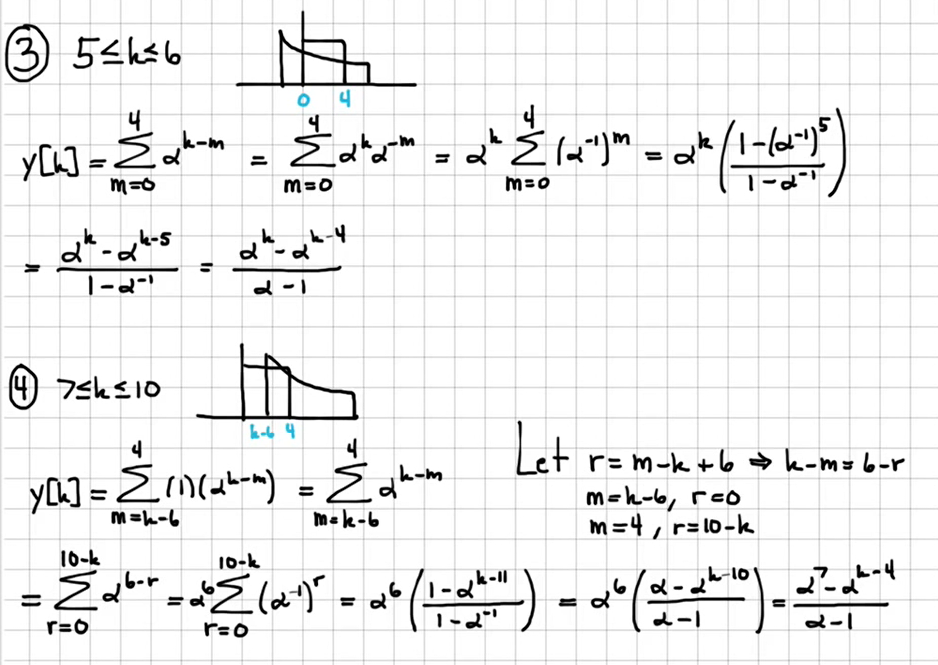
\includegraphics[width = 0.7\textwidth, frame]{Figures/Convolution/Example_2_SlidingTapes_Cases_2}
\caption{$5 \, \leq \, k \, \leq \, 6$ and $7 \, \leq \, k \, \leq \, 10$}
\label{fig:Convolution:Example_2_SlidingTapes_Cases_2}
\end{figure}

\newpage
\begin{figure}[h]
\centering
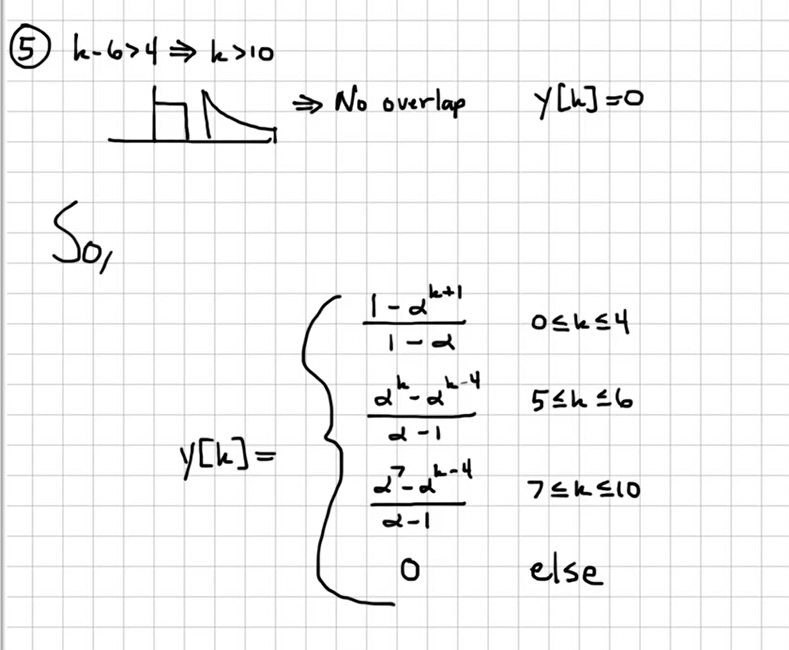
\includegraphics[width = 0.7\textwidth, frame]{Figures/Convolution/Example_2_SlidingTapes_Cases_3}
\caption{$k \, - \, 6 \, > \, 4$ and summing the cases}
\label{fig:Convolution:Example_2_SlidingTapes_Cases_3}
\end{figure}